\begin{figure}[h!]
    \centering
    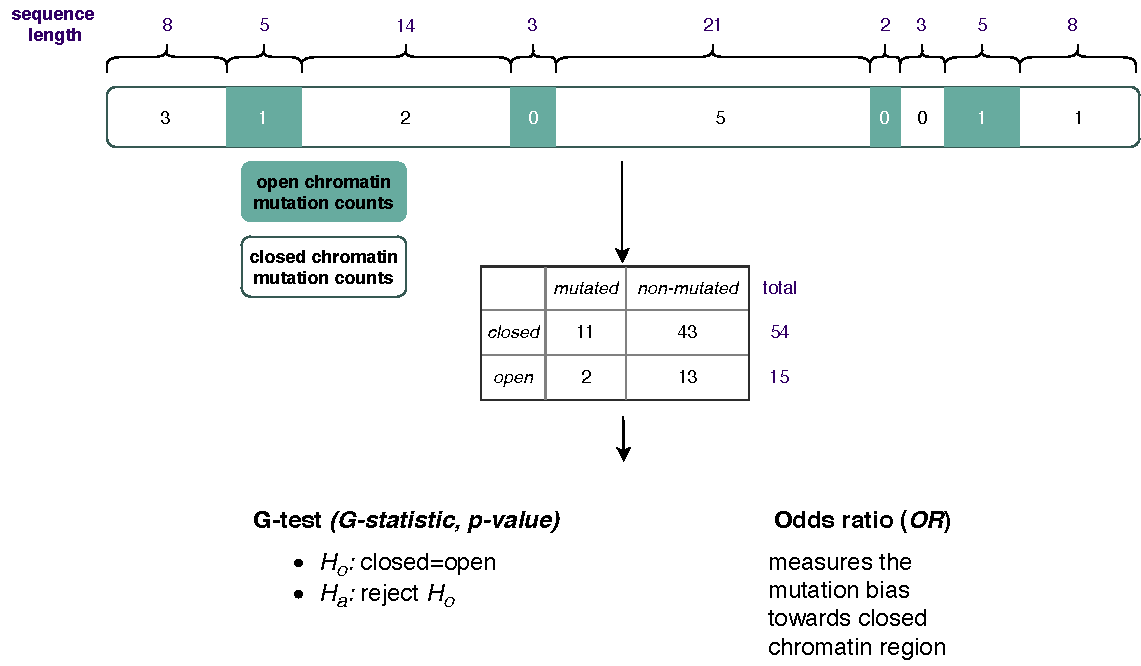
\includegraphics[scale=0.8]{graphics/mutdistribution.pdf}
    \caption{\textbf{Establishing the relationship between cancer mutation and chromatin structure of the original cell type.} Mutations were sorted into open and closed regions to make a contingency table, from which a G-test can be performed and an Odds-ratio ($OR$) statistic can be calculated. The G-test establishes whether there is a significant bias in mutation location; $OR$ measures the degree of bias towards closed chromatin regions.}
    \label{fig:gle_workflow}
\end{figure}
